% Created 2016-05-08 日 21:24
\documentclass[xcolor=svgnames,presentation]{beamer}
\usepackage[utf8]{inputenc}
\usepackage[T1]{fontenc}
\usepackage{fixltx2e}
\usepackage{graphicx}
\usepackage{longtable}
\usepackage{float}
\usepackage{wrapfig}
\usepackage{soul}
\usepackage{textcomp}
\usepackage{marvosym}
\usepackage{wasysym}
\usepackage{latexsym}
\usepackage{amssymb}
\usepackage{hyperref}
\tolerance=1000
\usepackage{minted}
\usecolortheme[named=FireBrick]{structure}\setbeamercovered{transparent}\setbeamertemplate{caption}[numbered]\setbeamertemplate{blocks}[rounded][shadow=true] \usetheme{Darmstadt}\date{\today} \usepackage{tikz}\usepackage{xeCJK}\usepackage{amsmath}\setmainfont{Times New Roman}\setCJKmainfont[BoldFont={Adobe Heiti Std},ItalicFont={Adobe Fangsong Std}]{Adobe Heiti Std}\setCJKsansfont{Adobe Heiti Std}\setCJKmonofont{Adobe Fangsong Std}\usepackage{verbatim}\graphicspath{{figures/}} \definecolor{lstbgcolor}{rgb}{0.9,0.9,0.9} \usepackage{listings}\usepackage{minted} \usepackage{fancyvrb}\usepackage{xcolor}\lstset{escapeinside=`',frameround=ftft,language=C,breaklines=true,keywordstyle=\color{blue!70},commentstyle=\color{red!50!green!50!blue!50},frame=shadowbox,backgroundcolor=\color{yellow!20},rulesepcolor=\color{red!20!green!20!blue!20}}
\usemintedstyle{default}
\providecommand{\alert}[1]{\textbf{#1}}

\title{第7讲 Linux系统配置与管理}
\author{王晓庆}
\date{\today}
\hypersetup{
  pdfkeywords={},
  pdfsubject={},
  pdfcreator={Emacs Org-mode version 7.9.3f}}

\institute{wangxiaoqing@outlook.com}
\begin{document}

\maketitle

\begin{frame}
\frametitle{Outline}
\setcounter{tocdepth}{1}
\tableofcontents
\end{frame}
\section{Linux系统启动过程与故障排除}
\label{sec-1}
\begin{frame}
\frametitle{Linux启动过程}
\label{sec-1-1}
\begin{columns}
\begin{column}{0.5\textwidth}
\begin{itemize}

\item Linux启动步骤
\label{sec-1-1-1}%
\begin{enumerate}
\item 启动BIOS
\item 启动引导
\item 启动内核
\item 启动并执行init程序
\end{enumerate}
\end{itemize} % ends low level
\end{column}
\begin{column}{0.5\textwidth}
%% Linux启动过程
\label{sec-1-1-2}

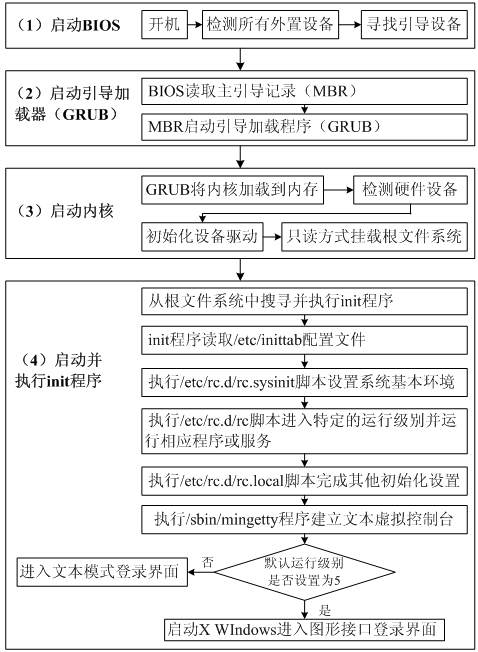
\includegraphics[width=.9\linewidth]{img/linuxboot.png}
\end{column}
\end{columns}
\end{frame}
\begin{frame}[fragile]
\frametitle{引导加载程序grub(1)}
\label{sec-1-2}
\begin{itemize}

\item /boot/grub/grub.conf(符号链接:/etc/grub.conf)\\
\label{sec-1-2-1}%
\begin{minted}[]{bash}
default=0 #默认启动的操作系统编号
timeout=5 #等待用户选择的时间(秒)
#引导菜单背景图案
splashimage=(hd0,0)/grub/splash.xpm.gz
hiddenmenu #隐藏引导菜单
title CentOS (2.6.18-398.e15) #引导项标题
        root (hd0,0)          #内核所在分区
        #内核文件及内核启动参数
        kernel /vmlinuz-2.6.18-398.e15 ro root=LABEL=/
        #内存磁盘镜像文件
        initrd /initrd-2.6.18-398.e15.img
\end{minted}
\end{itemize} % ends low level
\end{frame}
\begin{frame}
\frametitle{引导加载程序grub(2)}
\label{sec-1-3}
\begin{itemize}

\item 动态修改grub引导参数
\label{sec-1-3-1}%
\begin{itemize}

\item a \#添加引导参数
\label{sec-1-3-1-1}%

\item e \#编辑grub菜单
\label{sec-1-3-1-2}%

\item c \#进入grub命令行模式
\label{sec-1-3-1-3}%

\item 例:忘记root口令解决办法\\
\label{sec-1-3-1-4}%
在root行后加空格和1(或single)
\end{itemize} % ends low level

\item 设置grub密码
\label{sec-1-3-2}%
\begin{itemize}

\item 明文密码\\
\label{sec-1-3-2-1}%
password 明文密码

\item 加密密码
\label{sec-1-3-2-2}%
\begin{enumerate}
\item grub-md5-crypt生成加密密码
\item password --md5 加密密码
\end{enumerate}
\end{itemize} % ends low level
\end{itemize} % ends low level
\end{frame}
\begin{frame}
\frametitle{Linux运行级别}
\label{sec-1-4}

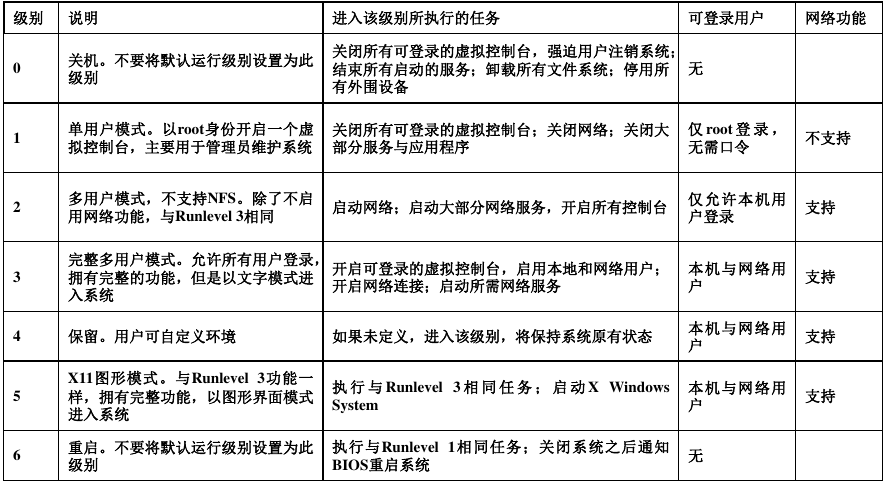
\includegraphics[width=.9\linewidth]{img/runlevels.png}
\end{frame}
\begin{frame}[fragile]
\frametitle{Linux运行级别}
\label{sec-1-5}
\begin{itemize}

\item 查看当前运行级别\\
\label{sec-1-5-1}%
\begin{minted}[]{bash}
runlevel
\end{minted}

\item 切换到不同的运行级别
\label{sec-1-5-2}%
\begin{itemize}

\item 启动时:通过grub将运行级别作为参数传给内核
\label{sec-1-5-2-1}%

\item 启动后:init或telinit
\label{sec-1-5-2-2}%
\end{itemize} % ends low level

\item 设置默认运行级别
\label{sec-1-5-3}%
\begin{itemize}

\item /etc/inittab文件中的参数id设置
\label{sec-1-5-3-1}%

\item 若未设置默认运行级别,启动过程中将提示用户输入一个运行级别
\label{sec-1-5-3-2}%
\end{itemize} % ends low level
\end{itemize} % ends low level
\end{frame}
\begin{frame}
\frametitle{init进程的工作过程}
\label{sec-1-6}
\begin{itemize}

\item init启动后,根据/etc/inittab文件的设置一次执行下列程序:
\label{sec-1-6-1}%
\begin{enumerate}
\item /etc/rc.d/rc.sysinit:初始化Linux系统的环境
\end{enumerate}
主要工作包括启动udev与SELinux系统,设置内核参数、系统时间、交换空间、主机名、检查并挂载必要但文件系统,初始化硬件设备,启用软磁盘阵列与LVM,卸载initrd,重设磁盘参数等。
\begin{enumerate}
\item /etc/rc.d/rc:建立并初始化运行级别环境
\end{enumerate}
不同的运行级别可提供不同的服务,通过/etc/rc.d/rc来启动或停止特定运行级别中的服务。
\begin{enumerate}
\item /etc/rc.d/rc.local:完成定制的初始化计划
\end{enumerate}
可在开机过程中执行某些初始化工作,执行该文件的前提是要进入的运行级别启用local服务,因为local服务的功能就是执行/etc/rc.d/rc.local

\item 管理员可以定制/etc/inittab来建立所需的系统运行环境
\label{sec-1-6-2}%
\end{itemize} % ends low level
\end{frame}
\begin{frame}[fragile]
\frametitle{/etc/inittab文件}
\label{sec-1-7}
\begin{itemize}

\item /etc/inittab文件格式\\
\label{sec-1-7-1}%
\begin{minted}[]{bash}
cat /etc/inittab
man 5 inittab
id:runlevels:action:process
id        #不超过4个字符的标识符
runlevels #运行级别列表,决定当前行对哪些运行级别起作用
action    #进程执行方式
  sysinit #只要系统引导就开始运行
  respawn #表示进程结束后重新启动该进程
  wait    #表示进程运行一次,init需要等待其运行结束
  initdefault #定义默认运行级别
process   #具体运行的进程
\end{minted}
\end{itemize} % ends low level
\end{frame}
\begin{frame}
\frametitle{系统启动过程故障排除顺序}
\label{sec-1-8}

\begin{enumerate}
\item 确定引导加载程序GRUB是否有问题
\item 检查是否正确载入kernel内核
\item 检查根目录是否挂载成功,如果不成功,应检查/sbin/init、/etc/inittab以及/boot/grub/grub.con配置文件的设置是否有错误,另外还要检查根目录是否损坏
\item 如果/etc/rc.d/rc.sysinit执行不成功,则有可能是/bin/bash文件损毁或是/etc/fstab配置有问题
\item 检查/etc/rc.d/rc以及/etc/rc.d/rc?.d(?表示运行级别)是否有问题
\end{enumerate}
\end{frame}
\begin{frame}
\frametitle{利用单用户模式修复系统(1)}
\label{sec-1-9}
\begin{itemize}

\item 单用户模式类型
\label{sec-1-9-1}%
\begin{enumerate}
\item runlevel 1
\end{enumerate}
执行init程序之后接着执行/etc/rc.sysinit程序以初始化系统,然后再执行/etc/rc1.d/目录下的所有程序
\begin{enumerate}
\item runlevel S
\end{enumerate}
执行init程序之后仅执行/etc/rc.sysinit程序以初始化系统
\begin{enumerate}
\item runlevel emergency
\end{enumerate}
执行init程序之后仅执行/etc/rc.sysinit程序中某些必要的程序,绕过rc.sysinit.sulogin,并不全部执行。
\end{itemize} % ends low level
\end{frame}
\begin{frame}
\frametitle{利用单用户模式修复系统(2)}
\label{sec-1-10}
\begin{itemize}

\item 进入单用户模式
\label{sec-1-10-1}%
\begin{itemize}

\item 在GRUB引导菜单按a或e键,根据需要在内核参数项上加上“1”或“single” ,以进入单用户模式
\label{sec-1-10-1-1}%

\item 在/etc/inittab配置文件将默认运行级别设置为1可在下次启动时进入单用户模式
\label{sec-1-10-1-2}%

\item 一个正在运行的Linux系统可以通过执行命令init 1切换至单用户模式
\label{sec-1-10-1-3}%

\item 启动至出现欢迎界面时,按下I键,系统会逐一询问是否启动每项服务,这时就处于runlevel S模式
\label{sec-1-10-1-4}%

\item 启动过程中如果挂载程序出现错误,会提示输入root用户密码,输入密码后,系统将直接进入runlevel emergency模式,完成修改后,按Ctrl-d将重启系统。
\label{sec-1-10-1-5}%
\end{itemize} % ends low level
\end{itemize} % ends low level
\end{frame}
\begin{frame}
\frametitle{利用单用户模式修复系统(3)}
\label{sec-1-11}
\begin{itemize}

\item 单用户模式修复的问题
\label{sec-1-11-1}%
\begin{itemize}

\item Runlevel 1执行至/etc/rc1.d/目录下的所有程序就结束,可以用来解决运行更高级别(2\~{}5)时所发生的错误
\label{sec-1-11-1-1}%

\item Runlevel S仅执行到rc.sysinit为止,除了可以解决Runlevel 1可以解决的问题之外,还可用来修复Runlevel 1发生的错误
\label{sec-1-11-1-2}%

\item RunLevel emergency除了Runlevel S可以解决的错误之外,还可以解决rc.sysinit发生的错误
\label{sec-1-11-1-3}%
\end{itemize} % ends low level
\begin{block}{注意}
\label{sec-1-11-1-4}

进入runlevel emergency时根文件系统处于只读状态,无法直接修改linux系统文件。假设/etc/fstab文件出了问题,启动时系统将进入emergency模式,这时需执行mount -o remount,rw /重新挂载根文件系统,以便对/etc/fstab进行修改。
\end{block}
\end{itemize} % ends low level
\end{frame}
\begin{frame}
\frametitle{使用Linux救援模式}
\label{sec-1-12}
\begin{itemize}

\item 救援模式(rescue mode)
\label{sec-1-12-1}%
\begin{itemize}

\item 当根目录所在的文件系统或grub损坏时无法启动内核或执行init进程,此时不能用单用户模式,而只能通过救援模式来修复linux系统故障。救援模式提供了从系统硬盘以外的设备(光盘、U盘等)引导一个小型linux环境的能力,引导成功后再对硬盘上的错误进行修改和恢复。
\label{sec-1-12-1-1}%
\end{itemize} % ends low level

\item 进入救援模式的几种方式
\label{sec-1-12-2}%
\begin{enumerate}
\item 从CentOS安装光盘的第1张盘引导系统
\item 从boot.iso映像制作的引导光盘引导系统
\item 从bookdisk.img映像制作的安装引导盘引导系统
\end{enumerate}
\end{itemize} % ends low level
\end{frame}
\begin{frame}
\frametitle{通过安装光盘进入Linux救援模式}
\label{sec-1-13}

\begin{enumerate}
\item 从光盘引导系统,出现boot:提示符后,输入linux rescue命令
\item 提示救援环境是图寻找硬盘中的linux系统,并将其挂载到/mnt/sysimage目录,需要选择如何处理(需要修改硬盘文件时选择Continue;仅需读取硬盘文件而不修改时选择Read-Only;如果要手动挂载文件系统则选择Skip直接跳过寻找并挂载硬盘的步骤。)
\item 按回车键后,系统提供一个shell给管理员使用
\item 进入救援模式后,正在运行的系统来自光盘,根分区也是光盘的/,硬盘分区全部被挂载到/mnt/sysimage目录,有些管理工具必须在硬盘环境中执行,这时需要利用chroot /mnt/sysimage命令将程序运行时的根目录改为硬盘根目录,完成修复后,执行exit退出chroot环境,因为在chroot环境中读不到光盘文件。
\end{enumerate}
\end{frame}
\begin{frame}[fragile]
\frametitle{实例:修复损坏的主引导记录}
\label{sec-1-14}
\begin{itemize}

\item 模拟损坏的主引导记录\\
\label{sec-1-14-1}%
\begin{minted}[]{bash}
dd if=/dev/zero of=/dev/sda bs=446 count=1
\end{minted}

\item 修复步骤
\label{sec-1-14-2}%
\begin{enumerate}
\item 用光盘引导系统,输入linux rescue进入救援模式
\item 改变根目录环境:chroot /mnt/sysinit
\item 修复主引导记录:grub-install /dev/sda
\item 执行exit退出chroot环境,再执行exit退出救援模式
\item 重新从硬盘引导系统
\end{enumerate}
\end{itemize} % ends low level
\note{如何修复分区表?

可百度testdisk,这是一款可以修复分区表和误删文件的Linux工具。
}
\end{frame}
\section{内核管理}
\label{sec-2}
\begin{frame}
\frametitle{内核组件}
\label{sec-2-1}
\begin{itemize}

\item 内核镜像文件
\label{sec-2-1-1}%
\begin{itemize}

\item 内核通常以镜像文件(Image File)形式存储在Linux系统中
\label{sec-2-1-1-1}%
\end{itemize} % ends low level

\item 内核模块
\label{sec-2-1-2}%
\begin{itemize}

\item Linux内核的功能可以编译到内核镜像文件中(静态模块),或者单独成为内核模块,以在系统运行期间动态地加载或者卸除模块(动态模块)
\label{sec-2-1-2-1}%
\end{itemize} % ends low level

\item initrd镜像文件
\label{sec-2-1-3}%
\begin{itemize}

\item Linux系统将部分模块制作成初始化内存磁盘(initrd)镜像文件, initrd文件是在系统引导过程中挂载的一个临时根文件系统,包含了引导过程中需要的模块和程序,可用来挂载实际的根文件系统。
\label{sec-2-1-3-1}%
\end{itemize} % ends low level
\end{itemize} % ends low level
\end{frame}
\begin{frame}
\frametitle{与内核有关的rpm软件包}
\label{sec-2-2}
\begin{itemize}

\item kernel:包括内核、内核模块和必要文件
\label{sec-2-2-1}%

\item kerenl-PAE:适用于物理内存超过4GB的内核软件包
\label{sec-2-2-2}%

\item kernel-xen:适用于Xen虚拟化系统的内核软件包
\label{sec-2-2-3}%

\item kernel-doc:Linux内核文档(内核源码的说明文件)
\label{sec-2-2-4}%

\item kernel-utils:提供Linux内核的管理工具,以及与内核有关的服务
\label{sec-2-2-5}%

\item kernel-TYPE-devel:编译不同类型的内核(内核镜像文件和模块)所需的文件,TYPE表示内核类型,如PAE
\label{sec-2-2-6}%
\end{itemize} % ends low level
\end{frame}
\begin{frame}
\frametitle{内核模块}
\label{sec-2-3}
\begin{itemize}

\item 可以在编译内核时选择将某些功能编译成为模块
\label{sec-2-3-1}%

\item 内核模块可使用户不用重新编译内核就可动态地启用或者停用某一项功能
\label{sec-2-3-2}%

\item 内核模块位于目录/lib/modules/`uname -r`/kernel
\label{sec-2-3-3}%
\begin{itemize}

\item arch:有关硬件平台
\label{sec-2-3-3-1}%

\item crypto:加密算法
\label{sec-2-3-3-2}%

\item drivers:硬件设备驱动程序
\label{sec-2-3-3-3}%

\item fs:有关文件系统
\label{sec-2-3-3-4}%

\item lib:各种模块所需用到的链接库
\label{sec-2-3-3-5}%

\item net:有关网络
\label{sec-2-3-3-6}%

\item sound:声卡驱动
\label{sec-2-3-3-7}%
\end{itemize} % ends low level

\item 模块文件的扩展名为.ko,文件名部分就是模块名称
\label{sec-2-3-4}%
\end{itemize} % ends low level
\end{frame}
\begin{frame}[fragile]
\frametitle{管理内核模块}
\label{sec-2-4}
\begin{itemize}

\item 查看已加载的内核模块\\
\label{sec-2-4-1}%
\begin{minted}[]{bash}
lsmod | grep md4
\end{minted}

\item 查看内核模块信息\\
\label{sec-2-4-2}%
\begin{minted}[]{bash}
modinfo [-0][-F 字段名] 模块名...
modinfo ext3
modinfo -F depends ext3
\end{minted}

\item 手动加载模块\\
\label{sec-2-4-3}%
\begin{minted}[]{bash}
insmod [模块文件名] [参数=值...]
insmod /lib/modules/`uname -r`/kernel/crypto/md4.ko
\end{minted}

\item 手动卸载模块\\
\label{sec-2-4-4}%
\begin{minted}[]{bash}
rmmod [-f] [-w] [-s] [-v] [模块名]
rmmod md4
\end{minted}
\end{itemize} % ends low level
\end{frame}
\begin{frame}[fragile]
\frametitle{处理模块间的依赖关系}
\label{sec-2-5}
\begin{itemize}

\item 使用modprobe命令可以自动加载或卸载所有必须用到的模块,modprobe从/lib/modules/`uname -r`/modules.dep文件读取模块的依赖关系。\\
\label{sec-2-5-1}%
\begin{minted}[]{bash}
modprobe [-C 配置文件] [模块名] [参数=值...]
modprobe md4 #默认配置文件为/etc/modprobe.conf
\end{minted}

\item 使用modprobe卸载模块只需使用-r选项\\
\label{sec-2-5-2}%
\begin{minted}[]{bash}
modprobe -r [模块名...]
\end{minted}

\item 使用选项-l显示符合条件的模块文件路径\\
\label{sec-2-5-3}%
\begin{minted}[]{bash}
modprobe -l [-t dirname] [wildcard]
modprobe -l tcp*
\end{minted}
\end{itemize} % ends low level
\end{frame}
\begin{frame}
\frametitle{内核模块配置文件}
\label{sec-2-6}
\begin{itemize}

\item /etc/modprobe.conf用于配置各种内核模块的值,主要功能是设置模块的默认参数,指定加载或卸载模块时要执行的任务,以及设置模块别名。
\label{sec-2-6-1}%
\begin{itemize}

\item alias:定义模块别名
\label{sec-2-6-1-1}%

\item options:设置模块默认参数
\label{sec-2-6-1-2}%

\item install:定义使用insmod或modprobe加载模块时执行的命令
\label{sec-2-6-1-3}%

\item remove:定义使用delmod或modprobe卸载模块时执行的命令
\label{sec-2-6-1-4}%

\item include:用于嵌入其他的内核模块配置文件
\label{sec-2-6-1-5}%
\end{itemize} % ends low level
\end{itemize} % ends low level
\end{frame}
\begin{frame}[fragile]
\frametitle{配置内核参数(1)}
\label{sec-2-7}
\begin{itemize}

\item 编辑/proc目录中的内核参数文件
\label{sec-2-7-1}%
\begin{itemize}

\item /proc/sys中的每一子目录存储重要的内核参数,这些目录中的每一个文件实际上是对应某一个内核参数,可称为内核参数文件,修改这些文件的内容就可以修改内核的功能\\
\label{sec-2-7-1-1}%
\begin{minted}[]{bash}
echo "server1.abc.com" >/proc/sys/kernel/hostname
\end{minted}

\item 修改内核参数属于临时修改,在关闭系统时就会丢失,可以通过修改/etc/rc.d/rc.local文件指定要设置哪些内核参数\\
\label{sec-2-7-1-2}%
\begin{minted}[]{bash}
echo 'echo "server1.abc.com" >\
/proc/sys/kernel/hostname' >>/etc/rc.d/rc.local
\end{minted}
\end{itemize} % ends low level
\end{itemize} % ends low level
\end{frame}
\begin{frame}[fragile]
\frametitle{配置内核参数(2)}
\label{sec-2-8}
\begin{itemize}

\item 使用sysctl配置内核参数
\label{sec-2-8-1}%
\begin{itemize}

\item sysctl定义的内核参数名称\\
\label{sec-2-8-1-1}%
\begin{minted}[]{bash}
/proc/sys/kernel/hostname对应内核参数kernel.hostname
\end{minted}

\item 查看内核参数\\
\label{sec-2-8-1-2}%
\begin{minted}[]{bash}
sysctl -a              #查看所有内核参数
sysctl kernel.hostname #查看指定内核参数
\end{minted}

\item 使用sysctl临时修改内核参数(立即生效)\\
\label{sec-2-8-1-3}%
\begin{minted}[]{bash}
sysctl -w kernel.hostname=server1
\end{minted}

\item 通过sysctl配置文件永久性配置内核参数\\
\label{sec-2-8-1-4}%
\begin{minted}[]{bash}
vim /etc/sysctl.conf    #默认内核参数配置文件
kernel.hostname=server1 #添加一行
sysctl -p               #使配置立即生效
\end{minted}
\end{itemize} % ends low level
\end{itemize} % ends low level
\end{frame}
\section{Linux软件包管理}
\label{sec-3}
\begin{frame}[fragile]
\frametitle{rpm软件包管理(1)}
\label{sec-3-1}
\begin{itemize}

\item rpm是由Red Hat公司提出的一种软件包管理标准,可用于软件的安装、查询、更新、升级、校验、卸载等。是目前应用比较广泛的软件包格式之一。
\label{sec-3-1-1}%

\item 另一个应用比较广泛的软件包格式是来自Debian Linux提出的deb软件包管理标准,其功能与rpm类似。
\label{sec-3-1-2}%

\item rpm软件包名称规范\\
\label{sec-3-1-3}%
\begin{minted}[]{bash}
name(名字)-version(版本)-release(发行).arch(架构).rpm
例:wget-1.11.4-3.el5_8.2.i386.rpm
\end{minted}
\end{itemize} % ends low level
\end{frame}
\begin{frame}[fragile]
\frametitle{rpm软件包管理(2)}
\label{sec-3-2}
\begin{itemize}

\item 安装\\
\label{sec-3-2-1}%
\begin{minted}[]{bash}
mount /dev/cdrom /media/cdrom
cd /media/cdrom/CentOS
rpm -ivh zsh-4.2.6-9.el5.i386.rpm
rpm -ivh --replacepkgs zsh-4.2.6-9.el5.i386.rpm #重新安装
\end{minted}

\item 升级\\
\label{sec-3-2-2}%
\begin{minted}[]{bash}
rpm -Uvh zsh-4.2.6-9.el5.i386.rpm
#会自动删除旧版软件包
#即使以前未安装过该软件包也会完成软件包的安装
#会自动把旧版本的配置文件备份
rpm -Uvh --oldpackage zsh-older.rpm #降级安装
\end{minted}

\item 卸载\\
\label{sec-3-2-3}%
\begin{minted}[]{bash}
rpm -e zsh-4.2.6-9.el5.i386.rpm
\end{minted}
\end{itemize} % ends low level
\end{frame}
\begin{frame}[fragile]
\frametitle{rpm软件包管理(3)}
\label{sec-3-3}
\begin{itemize}

\item 查询\\
\label{sec-3-3-1}%
\begin{minted}[]{bash}
rpm -qa      #打印所有已安装软件包列表
rpm -q zsh   #查询软件包是否安装
rpm -qa | grep zsh  #同上
rpm -qi zsh  #查看软件包信息
rpm -ql zsh  #查看软件包文件列表
rpm -qd zsh  #查看软件包文档列表
rpm -qc zsh  #查看软件包配置文件列表
rpm -qs zsh  #查看软件包文件状态
rpm -qf /etc/inittab #查询文件所属软件包
#上述带-q选项的命令加上-p选项可查询待安装rpm包信息
rpm -qip /media/cdrom/CentOS/w3m-0.5.1-18.el5.i386.rpm
\end{minted}
\end{itemize} % ends low level
\end{frame}
\begin{frame}[fragile]
\frametitle{rpm软件包管理(4)}
\label{sec-3-4}
\begin{itemize}

\item 校验\\
\label{sec-3-4-1}%
\begin{minted}[]{bash}
#rpm校验通常用于两种情况:
#1. 软件包本来运行良好,现在却出问题了,需要找出问题所在
#2. 安全性考虑,检查是否有关键文件被修改了
rpm -V pam
\end{minted}

\item rpm校验标记\\
\label{sec-3-4-2}%
\begin{center}
\begin{tabular}{ll}
 标记  &  相关属性      \\
\hline
 S     &  大小          \\
 M     &  模式(权限)    \\
 5     &  md5校验和     \\
 D     &  设备号不匹配  \\
 L     &  符号链接状态  \\
 U     &  所有者        \\
 G     &  所属组        \\
 T     &  修改时间      \\
\end{tabular}
\end{center}


\end{itemize} % ends low level
\end{frame}
\begin{frame}[fragile]
\frametitle{rpm软件包管理(5)}
\label{sec-3-5}
\begin{itemize}

\item 软件包签名验证
\label{sec-3-5-1}%
\begin{itemize}

\item CentOS公钥可以从以下任何一个地方获得:
\label{sec-3-5-1-1}%
\begin{itemize}
\item \href{http://mirror.centos.org/centos/}{http://mirror.centos.org/centos/}
\item 安装光盘根目录
\item /etc/pki/rpm-gpg/目录
\end{itemize}

\item 导入CentOS公钥\\
\label{sec-3-5-1-2}%
\begin{minted}[]{bash}
rpm --import /etc/pki/rpm-gpg/RPM-GPG-KEY-*
\end{minted}

\item 查看已导入的公钥列表\\
\label{sec-3-5-1-3}%
\begin{minted}[]{bash}
rpm -qa | grep gpg-pubkey
\end{minted}

\item 手动检查软件包签名\\
\label{sec-3-5-1-4}%
\begin{minted}[]{bash}
rpm --checksig evince-0.6.0-17.el5.i386.rpm
\end{minted}
\end{itemize} % ends low level
\end{itemize} % ends low level
\end{frame}
\begin{frame}[fragile]
\frametitle{rpm软件包管理(6)}
\label{sec-3-6}
\begin{itemize}

\item 高级查询\\
\label{sec-3-6-1}%
\begin{minted}[]{bash}
#查找系统已安装的10个最大软件包
rpm -qa --queryformat "%10{size} %{name}\n" \
| sort -rn | head
rpm -q --requires samba #查看samba软件包的必要条件
rpm -q --provides samba #查看samba软件包提供的内容
rpm -q --scripts samba  #查看samba软件包相关脚本
                        #相关脚本分为4类:
                        #安装前/安装后/卸载前/卸载后
rpm -qa --last | head   #查看最新安装的rpm软件包
\end{minted}
\end{itemize} % ends low level
\end{frame}
\begin{frame}[fragile]
\frametitle{rpm软件包管理(7)}
\label{sec-3-7}
\begin{itemize}

\item 从rpm包中提取文件\\
\label{sec-3-7-1}%
\begin{minted}[]{bash}
rpm2cpio 包全名 | cpio -idv .文件绝对路径
#rpm2cpio将rpm包转换为cpio格式
#cpio用于创建软件档案文件和从档案文件中提取文件
-i #copy-in模式,还原/提取
-d #还原时自动新建目录
-v #显示还原过程
\end{minted}
\end{itemize} % ends low level
\begin{exampleblock}{示例}
\label{sec-3-7-2}


\begin{minted}[]{bash}
rpm -qf /bin/cat      #查询cat属于哪个软件包
mv /bin/cat /tmp      #假装误删除cat命令
cd /mnt/cdrom/CentOS
rpm2cpio coreutils-5.97-34.el5_8.1.i386.rpm \|
cpio -idv ./bin/cat   #提取cat命令至当前目录
cp ./bin/cat /bin/cat #恢复cat命令至系统目录
\end{minted}
\end{exampleblock}
\end{frame}
\begin{frame}[fragile]
\frametitle{rpm软件包管理(8)}
\label{sec-3-8}
\begin{itemize}

\item rpm包的依赖性
\label{sec-3-8-1}%
\begin{itemize}

\item 树形依赖:a --> b --> c(可按c --> b --> a顺序安装解决)
\label{sec-3-8-1-1}%

\item 环形依赖:a --> b --> c --> a(可同时安装a、b、c解决)
\label{sec-3-8-1-2}%

\item 模块依赖:www.rpmfind.net(可查询模块所属软件包)\\
\label{sec-3-8-1-3}%
\begin{minted}[]{bash}
ldd /bin/cat #查看cat命令所需的动态链接库
\end{minted}
\end{itemize} % ends low level
\end{itemize} % ends low level
\begin{exampleblock}{rpm包依赖性示例}
\label{sec-3-8-2}


\begin{minted}[]{bash}
cd /mnt/cdrom/CentOS
rpm -ivh wireshark-gnome-1.0.15-6.el5_10.i386.rpm
\end{minted}
\end{exampleblock}
\end{frame}
\begin{frame}
\frametitle{yum包管理(1)}
\label{sec-3-9}
\begin{itemize}

\item yum(Yellowdog Update, Modified)是由Duke大学开发的包管理器,它能自动解决安装rpm软件包时遇到的依赖问题。
\label{sec-3-9-1}%
\begin{itemize}

\item 软件仓库:一个预先准备好的目录或网站,包含了软件包和索引文件。yum可以在仓库中自动定位并获取rpm软件包,只需一个命令就可以更新系统中的所有软件,也可以根据指定搜索条件来查找安装新的软件。
\label{sec-3-9-1-1}%

\item 配置yum仓库:在使用yum安装软件之前,应先配置yum指定使用的仓库。定义yum仓库的配置文件存放在/etc/yum.repos.d目录下,文件名格式为*.repo。
\label{sec-3-9-1-2}%
\begin{itemize}

\item 默认/etc/yum.repos.d目录内已经定义好了几个软件仓库。
\label{sec-3-9-1-2-1}%
\end{itemize} % ends low level
\end{itemize} % ends low level
\end{itemize} % ends low level
\end{frame}
\begin{frame}[fragile]
\frametitle{yum包管理(2)}
\label{sec-3-10}
\begin{itemize}

\item 配置本地yum源的步骤
\label{sec-3-10-1}%
\begin{itemize}

\item 建立yum软件仓库
\label{sec-3-10-1-1}%
\begin{enumerate}
\item 安装createrepo软件包
\item 将所有rpm软件包复制到一个目录(如/mnt/myrepo)
\item 执行createrepo /mnt/myrepo创建软件仓库
\end{enumerate}

\item 配置yum软件仓库
\label{sec-3-10-1-2}%
\begin{itemize}

\item 在/etc/yum.repos.d目录下建立myrepo.repo配置文件\\
\label{sec-3-10-1-2-1}%
\begin{verbatim}
[myrepo]
name=my local repo
baseurl=file:///mnt/myrepo
enabled=1
gpgcheck=1
gpgkey=file:///etc/pki/rpm-gpg/RPM-GPG-KEY-redhat-release
\end{verbatim}
\end{itemize} % ends low level

\item 清理yum缓存并导入签名\\
\label{sec-3-10-1-3}%
\begin{minted}[]{bash}
yum clean all
rpm --import /etc/pki/rpm-gpg/RPM-GPG-KEY-redhat-release
\end{minted}
\end{itemize} % ends low level
\end{itemize} % ends low level
\end{frame}
\begin{frame}[fragile]
\frametitle{yum包管理(3)}
\label{sec-3-11}
\begin{itemize}

\item yum软件包管理\\
\label{sec-3-11-1}%
\begin{minted}[]{bash}
yum list            #列出所有已安装和可用的软件包
yum list bash       #列出bash软件包
yum list available  #列出仓库中所有可用的软件包
yum list updates    #列出仓库中比已安装包更新的软件包
yum list installed  #列出已安装的软件包
yum list recent     #列出新加入仓库的软件包
yum search httpd    #搜索httpd相关软件包
yum -y install pkgs #安装软件包
yum -y update [pkgs]#升级软件包,未给包名则升级整个系统
yum remove pkgs     #删除软件包及所有依赖于该包的软件包
yum info pkgs       #查询软件包信息
yum grouplist       #查询软件包组
yum groupinstall "grpname" #安装软件包组
yum groupremove "grpname"  #卸载软件包组
\end{minted}
\end{itemize} % ends low level
\end{frame}
\begin{frame}[fragile]
\frametitle{yum包管理(4)}
\label{sec-3-12}
\begin{itemize}

\item 使用本地光盘yum源\\
\label{sec-3-12-1}%
\begin{minted}[]{bash}
mount /dev/cdrom /mnt/cdrom
cd /etc/yum.repos.d/
mkdir bak; mv *.repo bak; mv bak/CentOS-Media.repo .
vim CentOS-Media.repo
[c5-media]
name=CentOS-$releasever - Media
baseurl=file:///mnt/cdrom
#        file:///media/cdrom/
#        file:///media/cdrecorder/
gpgcheck=1
enabled=1
gpgkey=file:///etc/pki/rpm-gpg/RPM-GPG-KEY-CentOS-5
\end{minted}
注意:注释符\#必须位于行首!
\end{itemize} % ends low level
\end{frame}
\begin{frame}
\frametitle{源码包管理(1)}
\label{sec-3-13}
\begin{itemize}

\item 源码包
\label{sec-3-13-1}%
\begin{itemize}

\item 源码包大多以tar.gz和tar.bz2文件格式打包,里面包含源代码及相关文件
\label{sec-3-13-1-1}%

\item 源码包需要编译安葬,要求系统已安装开发工具和开发库
\label{sec-3-13-1-2}%
\begin{itemize}

\item 编译软件时可根据提示安装所需的开发工具和开发库,有时还要用源码包编译安装所依赖的包
\label{sec-3-13-1-2-1}%
\end{itemize} % ends low level

\item 通过rpm安装的包的相关信息在/var/lib/rpm中,可以通过rpm命令进行同一管理,而源码包则无法通过rpm命令进行管理
\label{sec-3-13-1-3}%

\item 通过rpm安装的包都是安装在默认位置,但源码包则可以安装在指定位置
\label{sec-3-13-1-4}%
\end{itemize} % ends low level
\end{itemize} % ends low level
\end{frame}
\begin{frame}
\frametitle{源码包管理(2)}
\label{sec-3-14}
\begin{itemize}

\item rpm包的默认安装位置\\
\label{sec-3-14-1}%
\begin{center}
\begin{tabular}{ll}
 /etc            &  配置文件安装目录    \\
 /usr/bin        &  可执行文件安装目录  \\
 /usr/lib        &  库文件安装目录      \\
 /usr/share/doc  &  软件文档安装目录    \\
 /usr/share/man  &  帮助手册安装目录    \\
\end{tabular}
\end{center}



\item 源码包一般安装位置\\
\label{sec-3-14-2}%
\emph{usr/local/软件名}
\end{itemize} % ends low level
\end{frame}
\begin{frame}[fragile]
\frametitle{源码包管理(3)}
\label{sec-3-15}
\begin{itemize}

\item rpm包安装的服务可以使用系统服务管理命令(service)进行管理,例如rpm包安装的apache的启动方法是:\\
\label{sec-3-15-1}%
\begin{minted}[]{bash}
/etc/rc.d/init.d/httpd start
service httpd start
\end{minted}
\begin{itemize}

\item 类似的命令有checkconfig、ntsysv等
\label{sec-3-15-1-1}%
\end{itemize} % ends low level

\item 源码包安装的服务不能被上述服务管理命令管理,因为没有安装到默认路径中,所以只能用绝对路径进行服务的管理\\
\label{sec-3-15-2}%
\begin{minted}[]{bash}
/usr/local/apache2/bin/apachectl start
\end{minted}
\end{itemize} % ends low level
\end{frame}
\begin{frame}
\frametitle{源码包管理(4)}
\label{sec-3-16}
\begin{itemize}

\item 源码包安装过程
\label{sec-3-16-1}%
\begin{enumerate}
\item 下载源码包
\item 解压缩源码包
\item 进入解压缩目录
\item 查看INSTALL和README文件
\item ./configure 软件配置与检查(编译前准备)
\begin{itemize}
\item 定义需要的功能选项(./configure --help查看可用选项)
\item 监测系统环境是否符合安装要求
\item 生成编译阶段所需的Makefile文件
\end{itemize}
\item 编译(make)
\begin{itemize}
\item 如果编译出错,在下一次重新编译前应该使用命令make clean 清空上次编译生成的文件
\end{itemize}
\item 编译安装(make install):需要root权限
\end{enumerate}
\end{itemize} % ends low level
\end{frame}
\begin{frame}[fragile]
\frametitle{源码包管理(5)}
\label{sec-3-17}
\begin{itemize}

\item 源码包安装示例\\
\label{sec-3-17-1}%
\begin{minted}[]{bash}
tar xjvf httpd-2.2.31.tar.bz2
cd httpd-2.2.31
vim INSTALL
./configure --prefix=/usr/local/apache2
make
make install
/usr/local/apache2/bin/apachectl start
/usr/local/apache2/bin/apachectl stop
\end{minted}

\item 源码包的卸载
\label{sec-3-17-2}%
\begin{itemize}

\item 不需要卸载命令,直接删除安装目录即可,不会遗留任何垃圾文件。\\
\label{sec-3-17-2-1}%
\begin{minted}[]{bash}
rm -rf /usr/local/apache2
\end{minted}
\end{itemize} % ends low level
\end{itemize} % ends low level
\end{frame}
\section{硬件管理}
\label{sec-4}
\begin{frame}
\frametitle{设备文件与设备识别号}
\label{sec-4-1}
\begin{itemize}

\item Linux内核并不关心/dev目录下的设备文件名,而是设备识别号
\label{sec-4-1-1}%

\item 每一个设备拥有主、次两个识别号
\label{sec-4-1-2}%
\begin{itemize}

\item 主识别号帮助操作系统查找设备驱动程序代码,区分设备种类
\label{sec-4-1-2-1}%

\item 次识别号用于区分同一类设备的不同个体,从0开始编号
\label{sec-4-1-2-2}%
\end{itemize} % ends low level

\item 设备识别号无法修改,除非修改Linux内核源码,并且重新编译内核
\label{sec-4-1-3}%
\end{itemize} % ends low level
\end{frame}
\begin{frame}[fragile]
\frametitle{创建设备文件}
\label{sec-4-2}
\begin{itemize}

\item mknod\\
\label{sec-4-2-1}%
mknod [选项] 设备文件名 类型 主识别号 次识别号

\begin{minted}[]{bash}
mknod /dev/md1 b 9 1
\end{minted}

\item MAKEDEV\\
\label{sec-4-2-2}%
根据/etc/makedev.d目录中的配置文件创建标准设备文件

\begin{minted}[]{bash}
cd /etc/makedev.d
grep 'sdb$' *
ls /dev/sd*
MAKEDEV -x sdb #-x 仅创建sdb,而非以sdb开头的所有设备
ls /dev/sd*
\end{minted}
\end{itemize} % ends low level
\end{frame}
\begin{frame}
\frametitle{通过udev自动创建设备文件}
\label{sec-4-3}
\begin{itemize}

\item 内核2.6版新增udev子系统,用于动态创建或删除设备文件,减少/dev目录的文件数
\label{sec-4-3-1}%

\item udev自动创建设备文件的过程
\label{sec-4-3-2}%
\begin{enumerate}
\item 内核发现安装/卸载某设备时,执行hotplug安装/卸载该硬件驱动程序
\item 请求执行udev创建/卸载该硬件的设备文件
\item udev通过libsysfs读取sys文件系统,获取该硬件设备信息
\item udev向namedev查询设备的设备文件信息,如名称、权限等
\item udev依据上述结果自动建立该设备的设备文件
\end{enumerate}

\item 如果需要修改系统预先提供的配置,可以修改/etc/udev目录中的udev规则配置文件
\label{sec-4-3-3}%
\begin{itemize}

\item udev主配置文件\\
\label{sec-4-3-3-1}%
/etc/udev/udev.conf 一般不用修改

\item udev规则文件:.rules文件\\
\label{sec-4-3-3-2}%
以两位数字开头,表示系统应用该规则的顺序。规则采用键-值对形式,一条规则由多个键值对组成,由逗号隔开。
\end{itemize} % ends low level
\end{itemize} % ends low level
\end{frame}
\begin{frame}[fragile]
\frametitle{监控硬件设备}
\label{sec-4-4}
\begin{itemize}

\item 内核事件信息
\label{sec-4-4-1}%
\begin{itemize}

\item 不管是Linux驱动硬件设备,还是硬件设备的状态发生变化,内核都会将这些信息存储为内核事件信息。
\label{sec-4-4-1-1}%

\item dmesg命令:可以查看存储于dmesg缓冲区的内容,但dmesg缓冲区仅能保存16K信息,一旦缓冲区满,新信息会覆盖最老的信息。
\label{sec-4-4-1-2}%

\item /var/log/dmesg文件:每次引导时会被重写,保存了最近一次启动后完整的内核事件信息
\label{sec-4-4-1-3}%
\end{itemize} % ends low level

\item 查看/proc相关文件\\
\label{sec-4-4-2}%
\begin{minted}[]{bash}
cat /proc/cpuinfo   #查看cpu信息
cat /proc/meminfo   #查看内存信息
cat /proc/devices   #查看硬件设备列表
cat /proc/diskstats #查看磁盘状态信息
/proc/ide/          #ide设备信息
/proc/scsi/         #scsi设备信息
\end{minted}
\end{itemize} % ends low level
\end{frame}
\begin{frame}[fragile]
\frametitle{管理PCI设备和USB设备}
\label{sec-4-5}
\begin{itemize}

\item 管理PCI设备\\
\label{sec-4-5-1}%
\begin{minted}[]{bash}
lspci  #查看系统安装的PCI设备信息
setpci [选项] 设备 操作 #配置PCI设备
\end{minted}
\end{itemize} % ends low level
\note{setpci

setpci命令使用举例:修改显示屏亮度
首先用lspci命令查看PCI设备
发现00:02.0是VGA设备,于是我们修改它的属性: 
sudo setpci -s 00:02.0 F4.B=FF
setpci 是修改设备属性的命令。 
-s 表示接下来输入的是设备的地址。 
00:02.0 VGA设备地址(<总线>:<接口>.<功能>)
F4 要修改的属性的地址,这里应该表示“亮度”
.B 修改的长度(B应该是字节(Byte),还有w(应该是Word,两个字节)、L(应该是Long,4个字节))
=FF 要修改的值(可以改)
我这里00是最暗,FF是最亮,不同的电脑可能不一样。
比如说我嫌FF太闪眼了,我就可以: 
sudo setpci -s 00:02.0 F4.B=CC
来自:\href{http://man.linuxde.net/setpci}{http://man.linuxde.net/setpci}
}
\begin{itemize}

\item 查看USB设备\\
\label{sec-4-5-3}%
\begin{minted}[]{bash}
lsusb                     #查看USB设备信息
cat /proc/bus/usb/devices #查看USB设备详细信息
\end{minted}
\end{itemize} % ends low level
\end{frame}
\section{系统性能监测}
\label{sec-5}
\begin{frame}
\frametitle{性能监测概述}
\label{sec-5-1}
\begin{itemize}

\item 性能监测的目的:找出系统的性能瓶颈以便调整优化
\label{sec-5-1-1}%

\item 系统性能指标
\label{sec-5-1-2}%
\begin{itemize}

\item 响应时间:从用户发出请求到用户得到返回结果所需时间
\label{sec-5-1-2-1}%

\item 吞吐量:在给定时间段内系统完成的交易数量
\label{sec-5-1-2-2}%
\end{itemize} % ends low level

\item 需监测的系统资源
\label{sec-5-1-3}%
\begin{itemize}

\item CPU
\label{sec-5-1-3-1}%

\item 内存
\label{sec-5-1-3-2}%

\item 磁盘
\label{sec-5-1-3-3}%

\item 网络
\label{sec-5-1-3-4}%
\end{itemize} % ends low level

\item 图形界面下的“系统监视器”,可以直观实时地查看进程、CPU、内存、网络和文件系统等方面的基本信息。但要深入分析系统性能,还需借助其他工具。
\label{sec-5-1-4}%
\end{itemize} % ends low level
\end{frame}
\begin{frame}[fragile]
\frametitle{CPU性能监测}
\label{sec-5-2}
\begin{itemize}

\item 安装sysstat软件包
\label{sec-5-2-1}%

\item sar命令显示CPU总的性能情况
\label{sec-5-2-2}%
\begin{itemize}

\item sar是后台进程sadc的前端显示工具,安装sysstat包后,sadc就会自动每隔10分钟收集一次系统状态并将它们存储到/var/log/sa目录中\\
\label{sec-5-2-2-1}%
\begin{minted}[]{bash}
sar [选项] [采样间隔] [采样次数]
sar   #查看当天的CPU统计信息
sar -u 3 5 #每3秒采样1次,连续采样5次
\end{minted}
\end{itemize} % ends low level

\item mpstat命令可查看多个CPU的情况\\
\label{sec-5-2-3}%
\begin{minted}[]{bash}
mpstat [-P CPU编号|ALL] [采样间隔] [采样次数]
mpstat
mpstat -P 0 3 5 #观测CPU0,每3秒采样1次,连续采样5次
\end{minted}
\end{itemize} % ends low level
\end{frame}
\begin{frame}[fragile]
\frametitle{内存和磁盘I/O性能监测}
\label{sec-5-3}
\begin{itemize}

\item 内存性能监测\\
\label{sec-5-3-1}%
\begin{minted}[]{bash}
free    #查看内存使用情况
sar -r  #查看内存统计信息
vmstat  #查看虚拟内存统计报告
\end{minted}

\item 磁盘I/O性能监测\\
\label{sec-5-3-2}%
\begin{minted}[]{bash}
sar -b  #查看磁盘I/O统计信息
iostat [选项] [采样间隔] [采样次数]
iostat
\end{minted}
\end{itemize} % ends low level
\end{frame}
\begin{frame}[fragile]
\frametitle{通过top实现综合监控}
\label{sec-5-4}
\begin{itemize}

\item top\\
\label{sec-5-4-1}%
\begin{minted}[]{bash}
top
us #用户进程占用CPU百分比
sy #系统内核占用CPU百分比
ni #更改过优先级的进程占CPU百分比
id #CPU空闲时间百分比
wa #CPU等待I/O操作时间百分比
hi #CPU用于处理硬件中断所占时间百分比
si #CPU用于处理软件中断所占时间百分比
st #虚拟设备所占CPU时间百分比
\end{minted}

\begin{verbatim}
PID(进程id) USER(用户) PR(优先级) NI(nice值)
VIRT(占用虚拟内存大小) RES(占用物理内存大小)
SHR(共享内存) S(进程状态) %CPU(占用CPU百分比)
%MEM(占用物理内存百分比) TIME+(使用CPU的时间)
COMMAND(进程命令名)
\end{verbatim}
\end{itemize} % ends low level
\end{frame}
\begin{frame}
\frametitle{优化系统性能}
\label{sec-5-5}

\begin{enumerate}
\item 使用监测工具监视系统的活动
\item 分析得到的性能数据,找出系统的性能瓶颈
\begin{itemize}
\item top默认按使用CPU百分比降序排列
\item 按M键可按内存占用百分比降序排列
\item 按F键可选择按任意字段排序或显示更多字段
\end{itemize}
\item 分析造成性能降低的原因,采取相应的优化措施
\begin{itemize}
\item 如果id值很低,说明CPU使用率很高,可以找出最占用CPU的进程
\item 如果wa值很高,说明系统处于高I/O状态,可用iostat进一步分析
\item 如果内存不足,可以找出最占用内存的进程
\end{itemize}
\end{enumerate}
\end{frame}
\section{系统日志管理}
\label{sec-6}
\begin{frame}
\frametitle{syslog简介}
\label{sec-6-1}

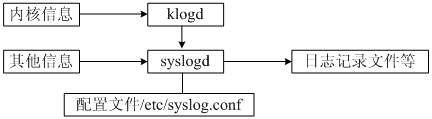
\includegraphics[width=.9\linewidth]{img/syslog.png}
\end{frame}
\begin{frame}
\frametitle{常见日志文件}
\label{sec-6-2}


\begin{center}
\begin{tabular}{ll}
 文件              &  记录内容                                  \\
\hline
 /var/log/cron     &  系统定时任务相关日志                      \\
 /var/log/cups     &  打印日志                                  \\
 /var/log/dmesg    &  系统开机时内核自检信息,可用dmesg查看     \\
 /var/log/btmp     &  错误登录日志,用lastb查看                 \\
 /var/log/lastlog  &  所有用户最后一次登录时间,用lastlog查看   \\
 /var/log/maillog  &  邮件日志                                  \\
 /var/log/message  &  系统绝大多数日志信息                      \\
 /var/log/secure   &  验证和授权日志,记录涉及账户和密码的操作  \\
 /var/log/wtmp     &  所有用户登录、系统启停日志,用last查看    \\
 /var/log/utmp     &  记录当前登录用户信息,用w、who等命令查看  \\
\end{tabular}
\end{center}
\end{frame}
\begin{frame}
\frametitle{常见日志文件(2)}
\label{sec-6-3}
\begin{itemize}

\item 除了系统默认的日志之外,采用rpm方式安装的系统服务也会默认把日志记录在/var/log/目录中(源码包安装的服务日志是在源码包指定目录中)。不过这些日志不是由syslogd服务来记录和管理的,而是各个服务使用自己的日志管理文档来记录自身日志。\\
\label{sec-6-3-1}%
\begin{center}
\begin{tabular}{ll}
 文件            &  记录内容                  \\
\hline
 /var/log/httpd  &  apache服务的服务日志目录  \\
 /var/log/mail   &  邮件服务的服务日志目录    \\
 /var/log/samba  &  samba服务的服务日志目录   \\
 /var/log/sssd   &  安全服务的服务日志目录    \\
\end{tabular}
\end{center}


\end{itemize} % ends low level
\end{frame}
\begin{frame}[fragile]
\frametitle{日志管理}
\label{sec-6-4}
\begin{itemize}

\item 日志格式
\label{sec-6-4-1}%
\begin{enumerate}
\item 时间产生的时间
\item 产生事件的服务器的主机名
\item 产生事件的服务名或程序名
\item 事件的具体信息
\end{enumerate}

\item 清空日志文件内容\\
\label{sec-6-4-2}%
\begin{minted}[]{bash}
echo >/var/log/secure
\end{minted}

\item /etc/syslog.conf配置文件\\
\label{sec-6-4-3}%
\begin{verbatim}
authpriv.* /var/log/secure
选择子      动作
选择子:服务名称[连接符号]日志等级
动作:日志记录位置或日志处理动作
认证相关服务.所有日志等级 记录在/var/log/secure中
\end{verbatim}
\end{itemize} % ends low level
\end{frame}
\begin{frame}
\frametitle{服务名称}
\label{sec-6-5}


\begin{center}
\begin{tabular}{ll}
 服务名称        &  含义                                        \\
\hline
 auth            &  安全和认证相关消息(不推荐使用authpriv替代)  \\
 authpriv        &  安全和认证相关消息(私有的)                \\
 cron            &  系统定时任务cron和at产生的日志              \\
 daemon          &  和各个守护进程相关的日志                    \\
 ftp             &  ftp守护进程产生的日志                       \\
 kern            &  内核而非用户进程产生的日志                  \\
 local10-local7  &  为本地使用预留的服务                        \\
 lpr             &  打印产生的日志                              \\
 mail            &  邮件收发日志                                \\
 news            &  与新闻服务器相关的日志                      \\
 syslog          &  由syslogd产生的日志信息                     \\
 user            &  用户等级类别的日志信息                      \\
 uucp            &  uucp子系统的日志信息                        \\
\end{tabular}
\end{center}
\end{frame}
\begin{frame}
\frametitle{日志等级}
\label{sec-6-6}


\begin{center}
\begin{tabular}{ll}
 等级名称  &  说明                                            \\
\hline
 none      &  不记录所有等级日志                              \\
 *         &  记录所有等级日志                                \\
 debug     &  一般的调试信息说明                              \\
 info      &  基本的通知信息                                  \\
 notice    &  普通信息,但是有一定的重要性                    \\
 warning   &  警告信息,但未影响到服务或系统的运行            \\
 err       &  错误信息,已经影响到服务或系统的运行            \\
 crit      &  临界状况信息,比err等级还要严重                 \\
 alert     &  警告状态信息,比crit还要严重,必须立即采取行动  \\
 emerg     &  紧急等级信息,系统已经无法使用                  \\
\end{tabular}
\end{center}
\end{frame}
\begin{frame}
\frametitle{连接符和日志处理方式}
\label{sec-6-7}
\begin{itemize}

\item 连接符\\
\label{sec-6-7-1}%
\begin{center}
\begin{tabular}{ll}
 连接符  &  含义                        \\
\hline
 .       &  记录大于等于指定等级的日志  \\
 .=      &  仅记录指定等级的日志        \\
 .!      &  记录除指定等级之外的日志    \\
\end{tabular}
\end{center}



\item 日志处理方式
\label{sec-6-7-2}%
\begin{itemize}

\item 记录至指定日志文件:如/var/log/secure
\label{sec-6-7-2-1}%

\item 发送到系统设备文件:如/dev/lp0
\label{sec-6-7-2-2}%

\item 转发给远程主机:如@192.168.0.210
\label{sec-6-7-2-3}%

\item 发送到指定用户所在终端:如root,adm
\label{sec-6-7-2-4}%
\end{itemize} % ends low level
\end{itemize} % ends low level
\end{frame}
\begin{frame}[fragile]
\frametitle{日志管理和测试}
\label{sec-6-8}
\begin{itemize}

\item 修改日志配置文件后使配置立即生效\\
\label{sec-6-8-1}%
\begin{minted}[]{bash}
killall -HUP syslogd
\end{minted}

\item 使用logger工具进行测试\\
\label{sec-6-8-2}%
\begin{minted}[]{bash}
logger kern.info "kern info test" #模拟kern.info消息
\end{minted}
\end{itemize} % ends low level
\end{frame}
\begin{frame}
\frametitle{日志轮替}
\label{sec-6-9}
\begin{itemize}

\item 日志轮替:防止日志占用过多磁盘空间
\label{sec-6-9-1}%
\begin{itemize}

\item 日志存储为多个文件,如每日一个
\label{sec-6-9-1-1}%

\item 限制日志文件个数,如只保留一周的日志
\label{sec-6-9-1-2}%
\end{itemize} % ends low level

\item 日志轮替中文件的命名规则\\
\label{sec-6-9-2}%
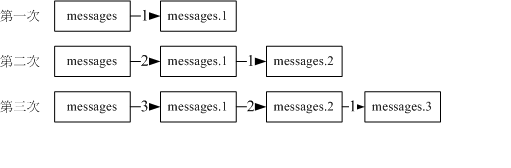
\includegraphics[width=.9\linewidth]{img/logrotate.png}
\end{itemize} % ends low level
\end{frame}
\begin{frame}
\frametitle{日志轮替配置文件/etc/logrotate.conf}
\label{sec-6-10}


\begin{center}
\begin{tabular}{ll}
 参数                     &  说明                                   \\
\hline
 daily                    &  每天轮替                               \\
 weekly                   &  每周轮替                               \\
 monthly                  &  每月轮替                               \\
 rotate n                 &  保留n个日志文件                        \\
 compress                 &  轮替时压缩旧日志                       \\
 create mode owner group  &  新建日志(权限、所有者、属组)           \\
 mail address             &  轮替时发邮件至指定邮箱地址             \\
 missingok                &  忽略日志不存在的情况                   \\
 notifempty               &  不轮替空日志                           \\
 minsize 10k              &  按时间轮替,日志小于10k时不轮替        \\
 size 1M                  &  日志按大小轮替,达到1M时轮替           \\
 dateext                  &  用日期作为日志后缀,如secure-20160606  \\
\end{tabular}
\end{center}
\end{frame}
\begin{frame}[fragile]
\frametitle{日志轮替管理}
\label{sec-6-11}
\begin{itemize}

\item 用rpm包安装的软件包默认使用了日志轮替
\label{sec-6-11-1}%

\item 用源码安装的软件包需要手工配置日志轮替\\
\label{sec-6-11-2}%
\begin{minted}[]{bash}
vim /etc/logrotate.conf
/usr/local/apache2/logs/access_log {
  daily
  create
  rotate 30
}
\end{minted}

\item logrotate [选项] 配置文件名
\label{sec-6-11-3}%
\begin{itemize}

\item 如果没有指定选项,则按照配置文件的配置进行日志轮替
\label{sec-6-11-3-1}%

\item -v 显示日志轮替详细信息
\label{sec-6-11-3-2}%

\item -f 强制进行日志轮替
\label{sec-6-11-3-3}%
\end{itemize} % ends low level
\end{itemize} % ends low level
\end{frame}
\begin{frame}[fragile]
\frametitle{集中式日志管理}
\label{sec-6-12}
\begin{itemize}

\item 在作为日志客户端的计算机上设置适当的信息传送到日志服务器。此时,需在“处理方式”字段中使用@指定日志服务器的计算机名称或IP地址\\
\label{sec-6-12-1}%
\begin{verbatim}
*.* @logserver
\end{verbatim}

\item 修改日志服务器的/etc/sysconfig/syslog配置文件\\
\label{sec-6-12-2}%
\begin{verbatim}
SYSLOGD_OPTIONS="-m 0 -r"
\end{verbatim}

\item 重新启动日志服务器与客户端的系统日志服务\\
\label{sec-6-12-3}%
\begin{minted}[]{bash}
service syslog restart
\end{minted}
\end{itemize} % ends low level
\end{frame}

\end{document}
